\documentclass[11pt,letterpaper]{article}
\usepackage[lmargin=1in,rmargin=1in,tmargin=1in,bmargin=1in]{geometry}
\usepackage{homework}

% -------------------
% Content
% -------------------
\begin{document}
\homework{Solutions --- Caleb McWhorter}

% Problem 1
\problem{10} Define a relation $\sim$ on $\mathbb{N} \times \mathbb{N}$ via $(x, y) \sim (a, b)$ if and only if $x - y= a - b$.  
        \begin{enumerate}[(a)]
        \item Is $(3, 1) \sim (2, 5)$? Explain.
        \item Is $(7, 3) \sim (5, 1)$? Explain. 
        \item Show that $\sim$ is an equivalence relation on $X$.
        \item Find at least 3 elements in each of the equivalence classes $[(1, 1)]$ and $[(3, 5)]$. 
        \end{enumerate} 

\sol 
\begin{enumerate}[(a)]
\item Let $(x, y)= (3, 1)$ and $(a, b)= (2, 5)$. Then $x - y= 3 - 1= 2$ and $a - b= 2 - 5= -3$. Because $x - y \neq a - b$, $(3, 1) \not\sim (2, 5)$. 

\item Let $(x, y)= (7, 3)$ and $(a, b)= (5, 1)$. Then $x - y= 7 - 3= 4$ and $a - b= 5 - 1= 4$. Because $x - y= a - b$, $(7, 3) \sim (5, 1)$. 

\item To show $\sim$ is an equivalence relation on $\mathbb{N} \times \mathbb{N}$, we need to show the relation is reflexive (for all $x \in X$, $x \sim x$), symmetric (if $x, y \in X$ and $x \sim y$, then $y \sim x$), and transitive (if $x, y, z \in X$, $x \sim y$, and $y \sim z$, then $x \sim z$):
	\begin{itemize}
	\item \textit{Reflexive:} Let $(x, y) \in \mathbb{N} \times \mathbb{N}$. We need to show that $(x, y) \sim (x, y)$. Observe that $x - y= 0= x - y$. Therefore, $(x, y) \sim (x, y)$. 
	
	\item \textit{Symmetric:} Let $(x, y), (a, b) \in \mathbb{N} \times \mathbb{N}$ and $(x, y) \sim (a, b)$. We need to show that $(a, b) \sim (x, y)$. Because $(x, y) \sim (a, b)$, we know that $x - y= a - b$. But then $a - b= x - y$. Therefore, $(a, b) \sim (x, y)$. 
	
	\item \textit{Transitive:} Let $(x, y), (a, b), (n, m) \in \mathbb{N} \times \mathbb{N}$ with $(x, y) \sim (a, b)$ and $(a, b) \sim (n, m)$. Because $(x, y) \sim (a, b)$, we know $x - y= a - b$. Similarly, because $(a, b) \sim (n, m)$, we know $a - b= n - m$. But then $x - y= a - b= n - m$, so that $x - y= n - m$. Therefore, $(x, y) \sim (n, m)$. 
	\end{itemize} \pspace

\item If $(x, y) \in [(1, 1)]$, then $x - y= 1 - 1= 0$. But then $x - y= 0$ so that $x= y$. Clearly, if $x= y$, then $x - y= 0= 1 - 1$ so that $(x, y) \in [(1, 1)]$. Therefore, $(x, y) \in [(1, 1)]$ if and only if $x= y$. This shows the elements of $[(1, 1)]$ are of the form $(x, x)$, where $x \in \mathbb{N}$. This shows that $[(1, 1)]= \{ (x, x) \colon x \in \mathbb{N}$. But then, for example, $(1, 1), (2, 2), (15, 15), (23^{23}, 23^{23}) \in [(1, 1)]$. 

\item If $(x, y) \in [(3, 5)]$, then $x - y= 3 - 5= - 2$. But then $x - y= -2$ so that $x= y - 2$. Suppose $x= y - 2$. Because $x \in \mathbb{N}$, $x \geq 1$. As $x= y - 2$, we know that $x= y - 2 \geq 1$. But then $y \geq 3$. Clearly, if $x= y - 2$, then $x - y= (y - 2) - y= -2= 3 - 5$ so that $(x, y) \in [(3, 5)]$. Therefore, $(x, y) \in [(3, 5)]$ if and only if $x= y - 2$ and $y \geq 3$. This shows the elements of $[(3, 5)]$ are of the form $(x, y)= (y - 2, y)$, where $y \geq 3$. Therefore, $[(3, 5)]= \{ (y - 2, y) \colon y \in \mathbb{N}, y \geq 3 \}$. But then, for example, $(3, 5), (4, 6), (10, 12), (103, 105) \in [(3, 5)]$. 
\end{enumerate}



\newpage



% Problem 2
\problem{10}  Define a relation on $\mathbb{R}$ via $x \sim y$ if and only if $x \leq y$. Prove or disprove whether $\sim$ is an equivalence relation on $\mathbb{R}$. \pspace

\sol We prove that $\sim$ is \textit{not} an equivalence relation on $\mathbb{R}$. If $\sim$ were an equivalence relation on $\mathbb{R}$, we would need to show the relation is reflexive (for all $x \in X$, $x \sim x$), symmetric (if $x, y \in X$ and $x \sim y$, then $y \sim x$), and transitive (if $x, y, z \in X$, $x \sim y$, and $y \sim z$, then $x \sim z$):
	\begin{itemize}
	\item \textit{Reflexive:} Let $x \in \mathbb{R}$. We need to show that $x \sim x$. But $x \leq x$ so that $x \sim x$. Therefore, $\sim$ is a reflexive relation on $\mathbb{R}$. 
	
	\item \textit{Symmetric:} Let $x, y \in \mathbb{R}$ with $x \sim y$. We need to show that $y \sim x$. Because $x \sim y$, we know that $x \leq y$. However, it need not be the case that $y \leq x$, implying $y \sim x$. For instance, we know that $1 \sim 3$ because $1 \leq 3$. But $3 \not\leq 1$ so that $3 \not\sim 1$. Observe that if $x \sim y$, then $x \leq y$, and if $y \sim x$, then $y \leq x$. But then $x \sim y$ and $y \sim x$ implies that $x \leq y$ and $y \leq x$ so that $x= y$. Clearly, if $x= y$, then $x \sim y$ and $y \sim x$. Therefore, $x \sim y$ and $y \sim x$ if and only if $x= y$. The relation $\sim$ on $\mathbb{R}$ is only symmetric only for the equal elements in $\mathbb{R}$. 
	
	\item \textit{Transitive:} Let $x, y, z \in \mathbb{R}$ with $x \sim y$ and $y \sim z$. We need to show that $x \sim z$. Because $x \sim y$, we know $x \leq y$. Furthermore, because $y \sim z$, we know $y \leq z$. But then $x \leq y \leq z$ so that $x \leq z$. This shows that $x \sim z$. Therefore, $\sim$ is a transitive relation on $\mathbb{R}$. 
	\end{itemize}

Despite the fact that $\sim$ is a reflexive and transitive relation on $\mathbb{R}$, $\sim$ is \textit{not} an equivalence relation on $\mathbb{R}$ because $\sim$ is not symmetric on $\mathbb{R}$. 



\newpage



% Problem 3
\problem{10} Define a relation on $\mathbb{R}^2$ via $(x, y) \sim (a, b)$ if and only if $(x, y)$ and $(a, b)$ are the same distance from the origin. 
	\begin{enumerate}[(a)]
	\item Prove that $\sim$ is an equivalence relation.
	\item Explicitly find the equivalences classes as a set. 
	\item Describe the equivalence classes graphically. 
	\end{enumerate} \pspace

\sol 
\begin{enumerate}[(a)]
\item We know the distance, $d$, between two points, $(x, y)$ and $(a, b)$, in the place is given by $d= \sqrt{(x - a)^2 + (y - b)^2}$. Therefore, the distance from $(x, y)$ to the origin is $d= \sqrt{(x - 0)^2 + (y - 0)^2}= \sqrt{x^2 + y^2}$. To show $\sim$ is an equivalence relation on $\mathbb{R}^2= \mathbb{R} \times \mathbb{R}$, we need to show the relation is reflexive (for all $x \in X$, $x \sim x$), symmetric (if $x, y \in X$ and $x \sim y$, then $y \sim x$), and transitive (if $x, y, z \in X$, $x \sim y$, and $y \sim z$, then $x \sim z$):
	\begin{itemize}
	\item \textit{Reflexive:} Let $(x, y) \in \mathbb{R}^2$. We need to show that $(x, y) \sim (x, y)$. But it is clear that $(x, y)$ has the same distance to the origin as itself. Therefore, $(x, y) \sim (x, y)$. 
	
	\item \textit{Symmetric:} Let $(x, y), (a, b) \in \mathbb{R}^2$ and $(x, y) \sim (a, b)$. Because $(x, y) \sim (a, b)$, we know that $(x, y)$ has the same distance to the origin as $(a, b)$. But then it is immediate that $(a, b)$ has the same distance to the origin as $(x, y)$. Therefore, $(a, b) \sim (x, y)$. 
	
	\item \textit{Transitive:} Let $(x, y), (a, b), (r, s) \in \mathbb{R}^2$ with $(x, y) \sim (a, b)$ and $(a, b) \sim (r, s)$. Because $(x, y) \sim (a, b)$, we know $(x, y)$ and $(a, b)$ have the same distance to the origin, i.e. $\sqrt{x^2+ y^2}= \sqrt{a^2 + b^2}$. Because $(a, b) \sim (r, s)$, we know $(a, b)$ and $(r, s)$ have the same distance to the origin, i.e. $\sqrt{a^2 + b^2}= \sqrt{r^2 + s^2}$. But then $\sqrt{x^2 + y^2}= \sqrt{a^2 + b^2}= \sqrt{r^2 + s^2}$, which implies $\sqrt{x^2 + y^2}= \sqrt{r^2 + s^2}$. But then $(x, y)$ and $(r, s)$ have the same distance to the origin. Therefore, $(x, y) \sim (r, s)$. 
	\end{itemize} \pspace

\item Let $(a, b), (v, w) \in \mathbb{R}^2$ and suppose $(a, b) \in [(v, w)]$. Suppose that the distance from $(v, w)$ to the origin is $d  \in \mathbb{R}$, where $d \geq 0$. We know that $(a, b) \in [(v, w)]$ if and only if $(a, b)$ and $(v, w)$ have the same distance to the origin. But $(a, b)$ and $(v, w)$ have the same distance to the origin if and only if $d= \sqrt{a^2 + b^2}$. But $d= \sqrt{a^2 + b^2}$ if and only if $d^2= a^2 + b^2$. Therefore, $[(v, w)]= \{ (x, y) \in \mathbb{R}^2 \mid x^2 + y^2= d^2 \}$. \pspace

\item From (b), we know that $(a, b) \in [(v, w)]$ if and only if $d^2= a^2 + b^2$, where $d$ is the distance from $(v, w)$ to the origin. But $d^2= a^2 + b^2$ if and only if $(a, b)$ is a point on the circle $d^2= x^2 + y^2$, i.e. the circle of radius $d$ centered at the origin. That is, $[(v, w)]$ is the set of points on the circle centered at the origin that passes through the point $(v, w)$. This includes the `trivial circle $\{ (0, 0) \}$ (the origin), i.e. the circle with radius $0$ centered at the origin. 
\end{enumerate} \pspace

The work above shows $\sim$ partitions $\mathbb{R}^2$ into circles centered at the origin (including the `trivial circle' at the origin). 
	\[
	\fbox{
	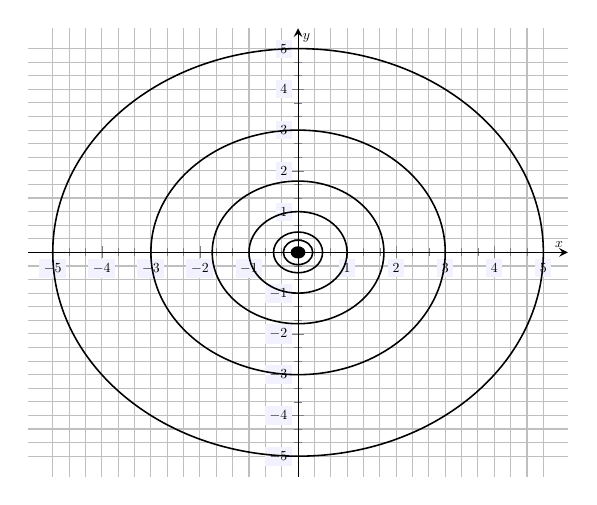
\begin{tikzpicture}[scale=1,every node/.style={scale=0.5}]
	\begin{axis}[
	grid=both,
	axis lines=middle,
	ticklabel style={fill=blue!5!white},
	xmin= -5.5, xmax=5.5,
	ymin= -5.5, ymax=5.5,
	xtick={-5,-4,...,5},
	ytick={-5,-4,...,5},
	minor x tick num= 2,
	minor y tick num= 2,
	xlabel=\(x\),ylabel=\(y\),
	]
	\draw[draw=none,fill=black] (0,0) circle (0.15);
	\pgfplotsinvokeforeach {0.3, 0.5, 1, 1.75, 3, 5} {
		\draw[line width=0.02cm] (0, 0) circle (#1);
	};
	
	\end{axis}
	\end{tikzpicture}
	}
	\]



\newpage



% Problem 4
\problem{10} Define a relation on $\mathbb{Z}$ via $a \sim b$ if and only if $a$ and $b$ have the same parity, i.e. $a$ and $b$ are either both even or they are both odd. 
        \begin{enumerate}[(a)]
        \item Show that $\sim$ is an equivalence relation. 
        \item Describe all the equivalence classes, i.e. determine the set $\mathbb{Z}/\sim$. 
        \end{enumerate} \pspace

\sol 
\begin{enumerate}[(a)]
\item To show $\sim$ is an equivalence relation on $\mathbb{Z}$, we need to show the relation is reflexive (for all $x \in X$, $x \sim x$), symmetric (if $x, y \in X$ and $x \sim y$, then $y \sim x$), and transitive (if $x, y, z \in X$, $x \sim y$, and $y \sim z$, then $x \sim z$):
	\begin{itemize}
	\item \textit{Reflexive:} Let $n \in \mathbb{Z}$. We need to show that $n \sim n$. But $n$ clearly has the same parity as $n$. Therefore, $n \sim n$.  
	
	\item \textit{Symmetric:} Let $n, m \in \mathbb{Z}$ with $n \sim m$. Because $n \sim m$, $n$ and $m$ have the same parity. But then $m$ has the same parity as $n$. Therefore, $n \sim m$. 
	
	\item \textit{Transitive:} Let $n, m, p \in \mathbb{Z}$ with $n \sim m$ and $m \sim p$. Because $n \sim m$, $n$ has the same parity as $m$. Because $m \sim p$, $m$ and $n$ have the same parity. But an integer cannot be both even an odd. Thus, $m$ has a fixed parity. The parity of $m$ from $n \sim m$ must then be the same parity of $m$ from $m \sim p$. But then because $n$ has the same parity as $m$, $n$ must have the same parity as $p$. Therefore, $n \sim p$. 
	\end{itemize} \pspace

\item Consider the equivalence class of $0 \in \mathbb{Z}$. We know that $0$ is even. But then if $n \in \mathbb{Z}$ is even, we know that $n \sim 0$. Therefore, $[0]= \{ \text{even integers} \}= \{ 2k \mid k \in \mathbb{Z} \}$. Now consider the equivalence class of $1 \in \mathbb{Z}$. We know that $1$ is odd. But then if $n \in \mathbb{Z}$ is odd, we know that $n \sim 1$. Therefore, $[1]= \{ \text{odd integers} \}= \{ 2k + 1 \mid k \in \mathbb{Z} \}$. If $n \in \mathbb{Z}$, then $n$ is either even or odd (but not both). But then $n \in [0]$ or $n \in [1]$. Therefore, $\mathbb{Z} / \sim= \{ [0], [1] \}$, i.e. there are only two equivalence classes:
	\[
	\begin{aligned}
	[0]&= \{ 2k \mid k \in \mathbb{Z} \}= \{ \text{even integers} \}=  \{ 0, \pm 2, \pm 4, \pm 6, \ldots \} \\[0.3cm]
	[1]&= \{ 2k + 1 \mid k \in \mathbb{Z} \}= \{ \text{odd integers} \}= \{ \pm 1, \pm 3, \pm 5, \pm 7, \ldots \}
	\end{aligned}
	\]
\end{enumerate}




\newpage





% Problem 5
\problem{10} Prove that if $X$ is a set and $S \subsetneq X$ is a nonempty subset of $X$, then $\{ S, X \setminus S \}$ is a partition of $X$. \pspace

\sol Let $X$ be a nonempty set and $\mathcal{A} \subseteq \mathcal{P}(S)$. Recall that $\mathcal{A}$ is a partition of $X$ if\dots
	\begin{itemize}
	\item $\varnothing \notin \mathcal{A}$
	\item $X= \bigcup_{A \in \mathcal{A}} A$
	\item For all $A, B \in \mathcal{A}$, if $A \neq B$, then $A \cap B= \varnothing$. 
	\end{itemize}
To prove that $\mathcal{A}= \{ S, X \setminus S \}$ is a partition of $X$, we need to check each of these conditions. 
	\begin{itemize}
	\item $\varnothing \notin \mathcal{A}$: There are only two distinct sets in $\bigcup_{A \in \mathcal{A}} A$---$S$ and $X \setminus S$. So we need only check that they are both nonempty. By assumption, $S$ is nonempty. Because $S \subsetneq X$, we know there exists $x \in X$ such that $x \notin S$. But then $x \in X \setminus S$, which implies that $X \setminus S \neq \varnothing$. \pspace
		
	\item $X= \bigcup_{A \in \mathcal{A}} A$: To show $X= \bigcup_{A \in \mathcal{A}} A$, we need to show that $X \subseteq \bigcup_{A \in \mathcal{A}} A$ and $\bigcup_{A \in \mathcal{A}} A \subseteq X$. We begin by showing $X \subseteq \bigcup_{A \in \mathcal{A}} A$. We need to show that if $x \in X$, then $x \in \bigcup_{A \in \mathcal{A}} A$. Let $x \in X$. Either $x \in S$ or $x \notin S$. But then either $x \in S$ or $x \in X \setminus S$, respectively. But then\dots
		\[
		x \in S \cup (X \setminus S)= \bigcup_{A \in \mathcal{A}} A
		\] 
	This proves that $X \subseteq \bigcup_{A \in \mathcal{A}} A$. Now we need to show that $\bigcup_{A \in \mathcal{A}} A \subseteq X$, i.e. we need to show that if $x \in \bigcup_{A \in \mathcal{A}} A$, then $x \in X$. If $x \in \bigcup_{A \in \mathcal{A}} A= S \cup (X \setminus S)$, then either $x \in S$ or $x \in X \setminus S$. But $S \subseteq X$ and $X \setminus S \subseteq X$. But then either $x \in S \subseteq X$ or $x \in X \setminus S \subseteq X$. This implies that $x \in X$, so that $\bigcup_{A \in \mathcal{A}} A \subseteq X$. Because $X \subseteq \bigcup_{A \in \mathcal{A}} A$ and $\bigcup_{A \in \mathcal{A}} A \subseteq X$, we know that $X= \bigcup_{A \in \mathcal{A}} A$. \pspace
	
	\item For all $A, B \in \mathcal{A}$, if $A \neq B$, then $A \cap B= \varnothing$: There are only two distinct sets in $\bigcup_{A \in \mathcal{A}} A$---$S$ and $X \setminus S$. So we need only check that $S \cap (X \setminus S)= \varnothing$. Suppose that $x \in S \cap (X \setminus S)$. This implies that $x \in S$ and $x \in X \setminus S$. Because $x \in X \setminus S$, we know that $x \in X$ and $x \notin S$. This contradicts the fact that $x \in S$. Therefore, $S \cap (X \setminus S)= \varnothing$. \pspace
	\end{itemize}



\newpage



% Problem 6
\problem{10} Let $X$ be a nonempty set. Every equivalence relation $\sim$ on $X$ gives rise to a partition on $X$. Moreover, every partition on $X$ gives rise to an equivalence relation $\sim$ on $X$. We proved the first statement in class. Suppose that $\{ X_i \}_{i \in \mathcal{I}}$ is a partition of $X$. Show that this partition induces an equivalence relation $X/\sim$ given by $a \sim b$ if and only if $a, b \in X_i$ for some $i \in \mathcal{I}$. \pspace

\sol Assume that $\{ X_i \}_{i \in \mathcal{I}}$ is a partition of a set $X$. Let $\sim$ be the relation on $X$ given by the following: if $a, b \in X$, then $a \sim b$ if and only if $a, b \in X_i$ for some $i \in \mathcal{I}$. To show $\sim$ is an equivalence relation on $X$, we need to show the relation is reflexive (for all $x \in X$, $x \sim x$), symmetric (if $x, y \in X$ and $x \sim y$, then $y \sim x$), and transitive (if $x, y, z \in X$, $x \sim y$, and $y \sim z$, then $x \sim z$):
	\begin{itemize}
	\item \textit{Reflexive:} Let $x \in X$. We need to show that $x \sim x$. Because $\{ X_i \}_{i \in \mathcal{I}}$ is a partition of $X$, we know that $X= \bigcup_{i \in \mathcal{I}} X_i$. Therefore, $x \in X= \bigcup_{i \in \mathcal{I}} X_i$. Therefore, there exists $i \in \mathcal{I}$ such that $x \in X_i$. Because $x, x \in X_i$, we know that $x \sim x$.\footnote{\label{PartitionFootnote}This only used the $X= \bigcup_{A \in \mathcal{A}} A$ property of a partition.} \par\vspace{0.2cm}
	
	\item \textit{Symmetric:} Let $x, y \in X$ with $x \sim y$. We need to show that $y \sim x$. Because $x \sim y$, we know there exists $i \in \mathcal{I}$ such that $x, y \in X_i$. But then $y, x \in X_i$. Therefore, $y \sim x$.\footref{PartitionFootnote} \par\vspace{0.2cm}
	
	\item \textit{Transitive:} Let $x, y, z \in X$ with $x \sim y$ and $y \sim z$. We need to show that $x \sim z$. Because $x \sim y$, there exists $i \in \mathcal{I}$ such that $x, y \in X_i$. Similarly, because $y \sim z$, there exists $j \in \mathcal{I}$ such that $y, z \in X_j$. We know $y \in X_i$ and $y \in X_j$ so that $y \in X_i \cap X_j$. If $i \neq j$, then $X_i \cap X_j \neq \varnothing$ because $y \in X_i \cap X_j$, contradicting the fact that $\{ X_i \}_{i \in \mathcal{I}}$ is a partition of $X$. Therefore, $i= j$. But then $z \in X_i= X_j$. This shows that $x, z \in X_i$. Therefore, $x \sim z$. 	
	\end{itemize} 

For completeness, we will also include the proof that every equivalence relation $X/\sim$ gives a partition of $X$---namely, the collection $\mathcal{P}:= \{ [x] \colon x \in X \}$, i.e. the set of equivalence classes form a partition of $X$. To show this is a partition, we must show the following:
	\begin{itemize} \itemsep= 0ex
	\item $\varnothing \notin \mathcal{P}$
	\item $X= \bigcup_{A \in \mathcal{P}} A$
	\item For all $A, B \in \mathcal{P}$, if $A \neq B$, then $A \cap B= \varnothing$. 
	\end{itemize}
We check each condition individually.
	\begin{itemize}
	\item $\varnothing \notin \mathcal{P}$: Let $A \in \mathcal{P}$. Because $A \in \mathcal{P}$, we know $A= [x]$ for some $x \in X$. But $x \in [x]$ so that $x \in A$. Therefore, $A \neq \varnothing$. 
	\item $X= \bigcup_{A \in \mathcal{P}} A$: To prove $X= \bigcup_{A \in \mathcal{P}} A$, we need to prove that $\bigcup_{A \in \mathcal{P}} A \subseteq X$ and $X \subseteq \bigcup_{A \in \mathcal{P}} A$. First, we prove that $\bigcup_{A \in \mathcal{P}} A \subseteq X$. Observe that for all $A \in \bigcup_{A \in \mathcal{P}} A$, $A= [x]$ for some $x \in X$. But then $A= [x] \subseteq X$. Because $A \subseteq X$ for all $A \in \bigcup_{A \in \mathcal{P}} A$, it must be that $\bigcup_{A \in \mathcal{P}} A \subseteq X$. Now we need to prove that $X \subseteq \bigcup_{A \in \mathcal{P}} A$. Let $x \in X$ and define $A= [x]$. We know that $x \in [x]= A$. But $A \subseteq \bigcup_{A \in \mathcal{P}} A$ so that $x \in A \subseteq \bigcup_{A \in \mathcal{P}} A$. This implies that $x \in \bigcup_{A \in \mathcal{P}} A$. But then $x \in \bigcup_{A \in \mathcal{P}} A$ for all $x \in X$. Therefore, $X \subseteq \bigcup_{A \in \mathcal{P}} A$. 
	\item For all $A, B \in \mathcal{P}$, if $A \neq B$, then $A \cap B= \varnothing$: Let $A, B \in \bigcup_{P \in \mathcal{P}} P$. Then there exist $x, y \in X$ such that $A= [x]$ and $B= [y]$. Because $A= [x]$ and $B= [y]$ are equivalence classes for $X/\sim$, we know that $A \cap B= [x] \cap [y]= \varnothing$ if and only if $[x]= [y]$, which happens if and only if $A= B$. Therefore, if $A \neq B$, we know that $A \cap B= \varnothing$.
	\end{itemize}








\end{document}